\chapter{Stokes Structures: Local}
\begin{comment}
  Matrizen Sicht:
  \begin{itemize}
    \item \cite[Chapter 3]{boalch}
      \\ largely following:
      \begin{itemize}
        \item[\textbf{8}] D.G. Babbitt and V.S. Varadarajan.
        \textbf{Formal reduction theory of meromorphic differential equations:
          a group theoretic view.}
        \texttt{euclid.pjm.1102720203.pdf}
        \item[\textbf{11}] W. Balser, W.B. Jurkat, and D.A. Lutz.
        \textbf{Birkhoff invariants and Stokes’ multipliers for meromorphic
          linear differential equations.}
        \item[\textbf{40}] M. Jimbo, T. Miwa, and Kimio Ueno.
        \textbf{Monodromy preserving deformations of linear differential
          equations with rational coefficients I.}
        \item[\textbf{43}] M. Loday-Richaud
        \textbf{Stokes phenomenon, multisummability and differential Galois
          groups.}
        \item[\textbf{50}] J. Martinet and J.P. Ramis.
        \textbf{Elementary acceleration and multisummability.}
      \end{itemize}
    \item \cite{thboalch}
    \item \cite{van2003galois}
    \item Marius van der Put, Kyoshi Saito => Diff.Galois Theory
  \end{itemize}
  Moderne Sicht (sheaf-view):
  \begin{itemize}
    \item Malgrange
    \item \cite{sabbah_cimpa90} and
    \item \cite{sabbah2007isomonodromic}
    \item \cite{sabbah2009introduction} and \cite{sabbah2013introduction}
  \end{itemize}
\end{comment}

\section{Matrix view: \cite{boalch} and \cite{thboalch}} %{{{
Let
\begin{itemize}
  \item $d-A^0$ be a diagonal meromorphic connection
    \begin{itemize}
      \item on the trivial rank $n$ vector bundle
        \begin{itemize}
          \item over the unit disc $\D\subset\C$
        \end{itemize}
      \item with a pole of order $k\geq2$ at $0$
        \begin{itemize}
          \item and no other poles.
        \end{itemize}
    \end{itemize}
  \item $z$ a coordinate on $\D$ vanishing at $0$.
\end{itemize}
Thus $A^0=dQ+\Lambda^0\frac{dz}{z}$ where
\begin{itemize}
  \item $\Lambda^0$ is a constant diagonal matrix and
  \item $Q$ is a diagonal matrix of meromorphic functions.
    \begin{itemize}
      \item write $Q=\diag(g_1,\dots,q_n)$
    \end{itemize}
\end{itemize}
Define $q_{ij}(z)$ to be the leading term of $q_i-q_j$.
\begin{itemize}
  \item Thus if $q_i-q_j=a/z^{k-1}+b/z^{k-2}+\dots$ then $q_{ij}=a/z^{k-1}$.
\end{itemize}
\subsection{Basic definitions}
\begin{defn}[Definition 3.2]
The \emph{anti-Stokes} directions $\A\subset S^1$ are the directions $d\in
S^1$ such that for some $i \neq j$: $q_{ij}(z)\in\R_{<0}$ for $z$ on the ray
specified by $d$.
\end{defn}
\begin{center}
  \begin{tikzpicture}[scale=2]
    \node[label=below left:$0$] (zero) at (0,0) {};
    \draw[blue] (zero) circle (1cm);
    \draw[red!60!black,thick,path fading=east] (0,0) -- +({cos( 33 )*2},{sin( 33 )*2});
    \fill[blue!20!white] ({cos( 33 )},{sin( 33 )}) circle (1pt);

    \node[blue] at (-0.9,0.6) {$S^1$};
    \node at (-1.3,-0.7) {$\C$};
    \node[blue!60!black,right] at ({cos( 33 )},{sin( 33 )}) {$d$};
    \node[red!60!black] at (2.2,.9) {ray specified by $d$};
    \fill (zero) circle (1pt);
  \end{tikzpicture}
\end{center}
\begin{itemize}
  \item We have $\frac{\pi}{k-1}$ rotational symmetry
    \begin{itemize}
      \item if $q_{ij}(z)\in\R_{<0}$ then
        $q_{ij}(z\exp(\frac{\pi\sqrt{-1}}{k-1}))\in\R_{<0}$
    \end{itemize}
  \item If $q_{ij}(z)\in\R_{<0}$ then $q_{ji}(z)\in\R_{>0}$
    \begin{itemize}
      \item in any arc $U \subset S^1$ subtending angle $\frac{\pi}{k-1}$
        there are at most $\frac{n(n-1)}{2}$ anti-Stokes directions.
    \end{itemize}
\end{itemize}
\begin{center}
  \begin{tikzpicture}[scale=3]
    \node[] (zero) at (0,0) {};
    \fill[fill=green!20!white] (0,0) -- (1,0) arc (0:60:1.0cm) -- cycle;
    \draw[blue] (zero) circle (1cm);

    \foreach \w/\str in {10/$d_1\in S^1$,
                         20/$d_2$,
                         45/$d_3$,
                         55/$d_l$}
    {\draw[thick,purple!\w!blue,path fading=west]
        (0,0) -- +({cos( \w )},{sin( \w )}) node[right] {\str};
     \fill[blue!20!white] ({cos( \w )},{sin( \w )}) circle (1pt);
     \foreach \sep in {60,120,180,240,300}
     {\draw[green!20!white,thick] (zero) -- +({cos( \sep )},{sin( \sep )});
      \draw[purple!\w!blue] (0,0) -- +({cos( \w + \sep )},{sin( \w + \sep )});
      \fill[blue!20!white] ({cos( \w + \sep )},{sin( \w + \sep )}) circle (1pt);
     }
    };

    \foreach \sep/\str in {0/$1$
                          ,60/$2$
                          ,120/$k-1$
                          ,180/$4$
                          ,240/$5$
                          ,300/$2(k-1)$}
    {\node[green!40!black]
      at ({.6 * cos( \sep + 30 )},{.5 * sin( \sep + 30)}) {\str};
    };

    \fill (zero) circle (1pt);
  \end{tikzpicture}
\end{center}
\begin{itemize}
  \item
    
\begin{tikzpicture}[scale=3]
      \fill[blue!20!white] (0,0) circle (1pt);
    \end{tikzpicture}
    $\in\A\subset S^1$ and $\#\A=:r$
    \begin{itemize}
      \item is divisible by $2(k-1)$ \Rightarrow{} $l:=\frac{r}{2k-2}$
    \end{itemize}
  \item $\textbf{d}=(d_1,d_2,d_3,\dots,d_l)\subset\A$ is a half-period
\end{itemize}
\begin{defn}
  \begin{itemize}
    \item $\Roots(d)=\{(ij)\mid g_{ij}(z)\in \R_{<0} \text{ along } d \}$
    \item The \emph{multiplicity} $\Mult(d)$ of $d$ is the number of roots
      supporting $d$.
    \item The group of \emph{Stokes factors} associated to $d$ is the group
    \[
      \mathbb{S}to_d(A^0) := \{K \in G \mid (K)_{ij}
        =\delta_{ij} \text{ unless } (ij) \text{ is a root of } d\}.
    \]
    \begin{itemize}
      \item $i=j$ \Rightarrow $(ij)$ is not a root of $d$. There are $1$nes
        on the diagonal.
      \item is a unipotent subgroup of $G=GL_n(\C)$ of dimension equal to the
        multiplicity of $d$
    \end{itemize}
    \item $n(n-1)/2=\Mult(d_1)+\dots+\Mult(d_l)$
  \end{itemize}
\end{defn}
\begin{defn}
  Define the open sector $\Sect(d_i,d_j)$
  \begin{center}
    \begin{tikzpicture}[scale=3]
      \node[] (zero) at (0,0) {};
      \draw[blue] (zero) circle (1cm);
      \fill[fill=green!20!white]
        (0,0) -- +({cos(10) * 0.7},{sin(10) * 0.7}) arc (10:45:0.7cm) -- cycle;
      \draw[->,thick,green!40!black] ({cos(10) * 0.7},{sin(10) * 0.7}) arc (10:45:0.7cm);

      \foreach \w/\str in {10/$d_1\in S^1$,
                           20/$d_2$,
                           45/$d_3$,
                           55/$d_l$}
      {\draw[thick,path fading=west] (0,0) -- +({cos( \w )},{sin( \w )}) node[right] {\str};
       \foreach \sep in {60,120,180,240,300}
       {\draw[gray] (0,0) -- +({cos( \w + \sep )},{sin( \w + \sep )});}
      };

      \fill (zero) circle (1pt);

      \node[green!40!black] at (1.2,0.6) {$\Sect(d_1,d_3)$};
      \node[green!40!black] at (0.4,0.02) {$r$};

    \end{tikzpicture}
  \end{center}
  \begin{itemize}
    \item The radius \textcolor{green!40!black}{$r$} will be taken sufficiently
      small when required later.
  \end{itemize}
\end{defn}
\[
  q_i\underset{\textbf{d}}{<}q_j \qquad :\Leftrightarrow
    \qquad (ij) \text{ is a root of some } d\in\textbf{d}
\]
Define permutation Matrix $P\in G$ associated do $\textbf{d}$ given by
$(P)_{ij}=\delta_{\pi(i)j}$ where
\begin{itemize}
  \item $\pi$ is the permutation of $\{1,\dots,n\}$ corresponding to
  \[
    q_i\underset{\textbf{d}}{<}q_j \qquad \Leftrightarrow \qquad \pi(i)<\pi(j)
  \]
\end{itemize}
\begin{lem}[3.2]
  \begin{enumerate}
    \item The product of the corresponding groups of Stokes factors is
    isomorphic as a variety, via the product map, to the subgroup of $G$
    conjugate to $U_+$ via $P$:
    \[
    \prod_{d\in\textbf{d}}\mathbb{S}to_d(A^0)\cong PU_+P^{-1} ;
    (K_1,\dots,K_l)\mapsto K_l\dots K_2K_1\in G
    \]
    \item Label the rest of $\A$ uniquely as $d_{l+1},\dots,d_r$ (in order)
    then the following map from the product of all the groups of Stokes
    factors, is an isomorphism of varieties:
    \[
    \prod_{d\in\A}\mathbb{S}to_d(A^0)\cong (U_+\times U_-)^{k-1} ;
    (K_1,\dots,K_r)\mapsto (S_1,\dots,K_{2k-2})
    \]
    \begin{itemize}
      \item where $S_i:=P^{-1}K_{il}\dots K_{(i-1)l+1}P\in U_{+/-}$ if $i$ is
      odd / even
    \end{itemize}
  \end{enumerate}
\end{lem}
Choose a point \textcolor{yellow!60!black}{$p$}\footnote{In~\cite{thboalch} a
sector is chosen, which does not contain any anti Stokes direction}
\begin{center}
  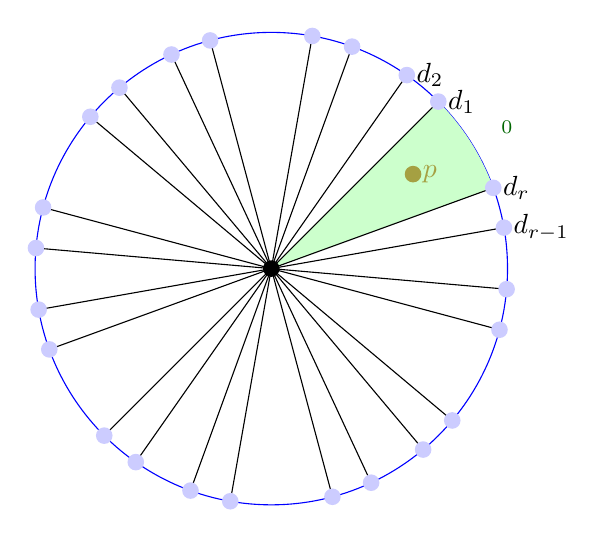
\begin{tikzpicture}[scale=3]
    \node[] (zero) at (0,0) {};
    \draw[blue] (zero) circle (1cm);

    \fill[fill=green!20!white] (0,0) -- ({cos( 20 )},{sin( 20 )}) arc
    (20:45:1) -- cycle;
    \node[green!40!black] at (1.0,0.6) {$\Sect_0$};

    \foreach \w/\str in {10/$d_{r-1}$,
                         20/$d_r$,
                         45/$d_1$,
                         55/$d_2$}
    {\draw (0,0) -- +({cos( \w )},{sin( \w )}) node[right] {\str};
     \fill[blue!20!white] ({cos( \w )},{sin( \w )}) circle (1pt);
     \foreach \sep in {60,120,180,240,300}
     {\draw (0,0) -- +({cos( \w + \sep )},{sin( \w + \sep )});
      \fill[blue!20!white]
        ({cos( \w + \sep )},{sin( \w + \sep )}) circle (1pt);
     }
    };

    \fill[yellow!60!black] (0.6,0.4) circle (1pt);
    \node[yellow!60!black,right] at (0.6,0.4) {$p$};

    \fill (zero) circle (1pt);
  \end{tikzpicture}
\end{center}
Label the first anti-Stokes ray when turning in a positive sense from $p$ as
$d_1$ and label the subsequent rays $d_2,\dots,d_r$ in turn.
\begin{itemize}
  \item Write $\Sect_i:= \Sect(d_i,d_{i+1})$ the ‘ith sector’.
  \begin{itemize}
    \item Note $p \in\Sect_r= \Sect_0$
  \end{itemize}
  \item $\widehat{\Sect}_i:=
    \Sect(d_i-\frac{\pi}{2k-2},d_{1+1}+\frac{\pi}{2k-2})$ the ‘ith supersector’
    \begin{itemize}
      \item The rays bounding these supersectors are usually refered as
        \textcolor{red!40!black}{‘Stokes rays’}.
    \end{itemize}
\end{itemize}
\begin{center}
  \begin{tikzpicture}[scale=3]
    \node[] (zero) at (0,0) {};
    \draw[blue] (zero) circle (1cm);

    \fill[fill=green!20!white] (0,0) -- ({cos( 15 )},{sin( 15 )}) arc
      (15:85:1) -- cycle;

    \fill[fill=red!60!black] (0,0) -- ({cos( 15 )*0.5},{sin( 15 )*0.5}) arc
      (15:45:0.5) -- cycle;
    \fill[fill=red!60!black] (0,0) -- ({cos( 55 )*0.5},{sin( 55 )*0.5}) arc
      (55:85:0.5) -- cycle;

    \fill[fill=green!20!white] (0,0) -- ({cos( 15 )*0.4},{sin( 15 )*0.4}) arc
      (15:85:0.4) -- cycle;

    \node[green!40!black] at (.9,.9) {$\widehat\Sect_1$};

    \node[] (lft) at ({cos( 85 )},{sin( 85 )}) {};
    \node[] (rgt) at ({cos( 15 )},{sin( 15 )}) {};

    \draw[->,red!40!black] ({cos( 45 )},{sin( 45 )})
      to [out=35, in=25] (rgt);

    \draw[->,red!40!black] ({cos( 55 )},{sin( 55 )})
      to [out=65, in=75] (lft);

    \draw[thick,red!40!black,path fading=west] (0,0) -- +({cos( 85 )},{sin( 85 )});
    \draw[thick,red!40!black,path fading=west] (0,0) -- +({cos( 15 )},{sin( 15 )});
    \fill[red!40!black] ({cos( 85 )},{sin( 85 )}) circle (1pt);
    \fill[red!40!black] ({cos( 15 )},{sin( 15 )}) circle (1pt);

    \foreach \w/\str in {10/$d_{r-1}$,
                         20/$d_r$,
                         45/$d_1$,
                         55/$d_2$}
    {\draw (0,0) -- +({cos( \w )},{sin( \w )}) node[right] {\str};
     \fill[blue!20!white] ({cos( \w )},{sin( \w )}) circle (.7pt);
     \foreach \sep in {60,120,180,240,300}
     {\draw (0,0) -- +({cos( \w + \sep )},{sin( \w + \sep )});
      \fill[blue!20!white]
        ({cos( \w + \sep )},{sin( \w + \sep )}) circle (.7pt);
     }
    };

    \fill[yellow!60!black] (0.6,0.4) circle (1pt);
    \node[yellow!60!black,right] at (0.6,0.4) {$p$};

    \fill (zero) circle (1pt);
  \end{tikzpicture}
\end{center}


\subsection{Theoremes}
\begin{thm}[1.22 in \cite{thboalch}]
  There is a natural isomorphism
  \[
    \cH(A^0)\cong\prod_{d\in\A}\Sto_d(A^0)
  \]
  and for each choice of $\log(z)$ in the direction $d$ the Stokes group
  $\Sto_d(A^0)$ has a faithfull representation $\rho$ on $\C^n$ inducing an
  isomorphism
  \[
    \rho:\Sto_d(A^0)\to\SSto_d(A^0).
  \]
  In particular each $\Sto_d(A^0)$ and therefore $\cH(A^0)$ is a unipotent Lie
  group and the complex dimension \dots
\end{thm}
\begin{thm}[3.1, or Prop 1.24 in \cite{thboalch}]
  Let $\hat{F}\in G\llbracket z\rrbracket$ such that $A:=F[A_0]$ has
  convergent entries.
  Set the radius of the sectors $\Sect_i$, $\widehat\Sect_i$ to be less than
  the radius of convergence of $A$.
  Then:
  \begin{enumerate}
    \item On each sector $\Sect_i$ there is a canonical way to choose an
      invertible $n\times n$ matrix of holomorphic Functions
      $\Sigma_i(\hat F)$ such that $\Sigma_i(\hat F)[A^0]=A$
    \item $\Sigma_i(\hat F)$ can be analytically continued to the supersector
      $\widehat\Sect_i$ and then $\Sigma_i(\hat F)$ is asymptotic to $\hat F$
      at $0$ within $\widehat\Sect_i$
    \item If $g\in G\{z\}$ and $t\in T$ then
      $\Sigma_i(g\circ\hat F \circ t^{-1})=g\circ\Sigma_i(\hat F)\circ t^{-1}$.
  \end{enumerate}
  \begin{rem}
    \begin{itemize}
      \item The point is that on a narrow sector there are generally many
        holomorphic isomorphisms between $A_0$ and $A$ which are asymptotic to
        $\hat F$ and one is being chosen in a canonical way
      \item $\Sigma_i(\hat F)$ is in fact uniquely characterised by property 2.
    \end{itemize}
  \end{rem}
\end{thm}
\begin{prop}[Prop 1.24 in \cite{thboalch}]
  \begin{enumerate}
  \setcounter{enumi}{2}
  \item If $\hat H\in\hat G$ is the taylor series at $0$ of an analytic gauge
    transformation $H\in G\{z\}$ then
    \[
      \Sigma_i(\hat H \hat F)=H\Sigma_i(\hat F)
      \qquad
      \Sigma_i(\hat F \hat H)=\Sigma_i(\hat F)H
    \]
  \end{enumerate}
\end{prop}
\begin{comment}
  \begin{rem}[1.41 from \cite{thboalch} on pages 16f]
    Note that in most of the recent references we have used, Stokes matrices
    are used to classify
    \begin{itemize}
      \item meromorphic connections within fixed formal \textbf{meromorphic
        classes, modulo meromorphic equivalence}.
    \end{itemize}
    Whereas here we classify
    \begin{itemize}
      \item meromorphic connections within fixed \textbf{formal analytic
        classes, modulo analytic equivalence},
    \end{itemize}
    as is done in the older literature.  The fact is that the sets equivalence
    classes are the same in both cases. It is important for us to work with
    analytic, rather than meromorphic gauge transformations, because then the
    $\C^\infty$ viewpoint in Chapter 3 is cleaner. This distinction relates to
    the difference between \textbf{‘regular singular’} connections and
    \textbf{‘logarithmic’} connections.
  \end{rem}
\end{comment}
%}}}

\section{Sheaf view: \cite{sabbah2007isomonodromic}} %{{{
Let
\begin{itemize}
  \item $X$ be a complex analytic manifold
    (\textcolor{green!40!black}{parameter space}) and
  \item $\cM^{good}$ be a meromorphic bundle on $D\times X$
    \begin{itemize}
      \item with poles along $\{0\}\times X$,
    \end{itemize}
    equipped with a flat connection $\nabla^{good}$.
\end{itemize}
We will assume that $\left(\sM^{good},\nabla^{good}\right)$ is 
\begin{itemize}
  \item a good model in the neighbourhood of $x^o$, that is that
    \begin{itemize}
      \item there exist pairwise distinct germs $\phi_1,\dots,\phi_p\in
        t^{-1}\cO_{X,x^o}[t^{-1}]$ and
      \item nonzero germs of systems with regular singularity
        $\cR_{\phi_1},\dots,\cR_{\phi_p}$ along $\{0\}\times X$ such that
            we have, in a neighbourhood of $x^o$,
        \begin{itemize}
          \item an isomorphism $\sM_{x^o}^{good}
            \cong\bigoplus_k\left(\cE^{\phi_k}\otimes\cR_{\phi_k}\right)$.
        \end{itemize}
    \end{itemize}
\end{itemize}
$k\neq l$ $\overset{\text{II.5.6}}{\Rightarrow{}}$ the order of the pole with
respect to $t$ of $(\phi_k-\phi_l)(x,t)$ does not depend on $x$ in a
neighbourhood of $x^o$.
\begin{defn}
  Define the \emph{stokes sheaf} $\St_X(\sM^{good})$ as the sheaf (on $X$)
  associated to the presheaf
  \[
    U\mapsto H^1(S^1\times U,\Aut^{<X}(\tilde \sM^{good}) )
  \]
  where
  \begin{itemize}
    \item $\Aut^{<\{0\}\times X}(\tilde M^{good})$ or
      $\Aut^{<X}(\tilde M^{good})$ is the sheaf
      \begin{itemize}
        \item on $S^1\otimes X$
        \item of auomorphisms of $\tilde M^{good}:=\cA_{\tilde D\times
          X}\otimes_{\cO_{D\times X}}\sM^{good}$
          witch are
          \begin{itemize}
            \item compatible with the connection and
            \item are formally equal to the identity\footnote{i.e., which
              induce the identity on $\hat \sM^{good}:=\hat \cO_{D\times
              X}\otimes_{\cO_{D\times X}}\sM^{good}$}.
          \end{itemize}
      \end{itemize}
      The sections of $\Aut^{<X}(\tilde M^{good})$ are called \emph{stokes
      matrices}.
  \end{itemize}
\end{defn}
\begin{thm}[The stokes sheaf is locally constant (6.1)]
  The Stokes sheaf $\St_X(\sM^{good})$ is
  \begin{itemize}
    \item a locally constant
  \end{itemize}
  sheaf of pointed sets.
\end{thm}
Let $(\sM,\nabla)$ be a meromorphic connection with
\begin{itemize}
  \item poles on $D\times X$ 
  \item flat connection, 
    \begin{itemize}
      \item having poles along $\{0\}\times X$.
    \end{itemize}
\end{itemize}
\begin{defn}
  $(\sM^{good},\nabla^{good})$ is a \emph{good formal model} for
  $(\sM,\nabla)$ if
  \begin{itemize}
    \item there exists an isomorphism 
      \[
        \hat f(\widehat\sM,\widehat\nabla)\overset{\sim}{\to}
        (\widehat{\sM^{good}},\widehat{\nabla^{good}})
      \]
      \begin{itemize}
        \item of sheafes of $\hat\cO_{D\times X}$-modules
        \item compatible with connection.
      \end{itemize}
  \end{itemize}
\end{defn}
\begin{defn}
  Two germs $(\sM,\nabla,\hat f)$ and $(\sM',\nabla',\hat f')$ along
  $\{0\}\times X$ are \emph{isomorphic}, if
  \begin{itemize}
    \item there exists an isomorphism\footnote{such an isomorphism then is
      unique} $g:(\sM,\nabla)\to(\sM',\nabla')$ with
      \begin{itemize}
        \item $\hat f=\hat f'\circ\hat g$.
      \end{itemize}
  \end{itemize}
\end{defn}
Let
\begin{itemize}
  \item $\sH_X$ be the (pre-) sheaf\footnote{Lemma 6.2: it is a sheaf.} where
    \begin{itemize}
      \item $\sH_X(U)$ is the set
        \begin{itemize}
          \item of isomorphism classes of germs $(\sM,\nabla,\hat f)$ defined
            on $U$,
          \item equipped with a distinguished element, namely, the class of
            ${(\sM^{good},\nabla^{good},\widehat{\Id})}_{|U}$.
        \end{itemize}
    \end{itemize}
\end{itemize}
\begin{thm}[The Stokes sheaf classifies meromorphic connections with fixed
  normal type (6.3)]
  The homomorphism so defined
  \[
    \sH_X\to St_X(\sM^{good})
  \]
  is an isomorphism of sheaves of pointed sets.
\end{thm}
%}}}

\section{Local Moduli}
\subsection{\dots / Models}

\subsection{\dots / Sectorial classificaton} %{{{
\begin{paracol}{2} %%%%%%%%%%%%%%%%%%%%%%%%%%%%%%%%%%%%%%%%%%%%%%%%%%%%%%%%%%%%
  \switchcolumn{} %%%%%%%%%%%%%%%%%%%%%%%%%%%%%%%%%%%%%%%%%%%%%%%%%%%%%%%%%%%%%
  Let $\cM$ be a germ at $(0,x^o)$ of a meromorphic bundle with poles along
  $\{0\}\times X$.
  \begin{thm}[II.5.12]
    Let us assume that there exists
    \begin{itemize}
      \item a good model $\cM^{good}$ and
      \item an isomorphism $\hat\lambda: \hat\cM
        \overset{\sim}{\longrightarrow}\hat\cM^{good}$.
    \end{itemize}
    Then,
    \begin{itemize}
      \item for any $e^{i\theta^o}\in S^1$,
    \end{itemize}
    there exists an isomorphism
    \[
      \tilde\lambda_{\theta^o}: \tilde\cM_{\theta^o}
      \overset{\sim}{\longrightarrow}\tilde\cM^{good}_{\theta^o},
    \]
    lifting $\hat\lambda$.
  \end{thm}
  That is, such that the diagram
  \[ \begin{tikzcd}
      \tilde\cM_{\theta^o} \dar \rar{\tilde\lambda_{\theta^o}} &
        \tilde\cM^{good}_{\theta^o} \dar
        \\\hat\cM \rar{\hat\lambda} &
        \hat\cM^{good}
  \end{tikzcd} \]
  commutes.
\end{paracol} %%%%%%%%%%%%%%%%%%%%%%%%%%%%%%%%%%%%%%%%%%%%%%%%%%%%%%%%%%%%%%%%%
%}}}

\chapter{Stokes Structures: Global}
\subsection{Situation} %{{{
\begin{paracol}{2} %%%%%%%%%%%%%%%%%%%%%%%%%%%%%%%%%%%%%%%%%%%%%%%%%%%%%%%%%%%%
  Fix the data $\textbf{a}$ of
  \begin{itemize}
    \item a Divisor $D=\sum k_i(a_i)$ on $\P^1$ and
    \item and connection germs $d-{}^iA^0$ at each $a_i$.
  \end{itemize}
  Let $(V,\nabla,\textbf{g})$ be a compatibly framed meromorphic connection on
  a holomorphic vector bundle $V\to\P^1$ with a irregular type $\textbf{a}$.

  \switchcolumn{} %%%%%%%%%%%%%%%%%%%%%%%%%%%%%%%%%%%%%%%%%%%%%%%%%%%%%%%%%%%%%
  Let
  \begin{itemize}
    \item $X$ be the parameter space
      \begin{itemize}
        \item an analytic manifold equipped with coordinates $x_1,\ldots,x_n$.
      \end{itemize}
    \item $\sM$ be a meromorphic bundle
      \begin{itemize}
        \item on $D\times X$
        \item with poles along $\{0\}\times X$
      \end{itemize}
      with \textbf{flat} connection
      \[
        \nabla:\sM\to\Omega_{D\times X}^1\otimes\sM
      \]
    \item $\cM$ denote its germ at $(0,x^0)\in D\times X$
      \begin{itemize}
        \item this is a module over the ring
          \[
            \cO_{D\times X,(0,x^0)}[t^{-1}]=\C\{t,x_1,\dots,x_n\}[t^{-1}]
          \]
      \end{itemize}
  \end{itemize}
\end{paracol} %%%%%%%%%%%%%%%%%%%%%%%%%%%%%%%%%%%%%%%%%%%%%%%%%%%%%%%%%%%%%%%%%
%}}}

